\section*{\ShortTitle}
\subsection*{Einleitung}
\begin{frame}
  \begin{center}
    \begin{figure}
      \begin{tikzpicture}
        \begin{scope} [fill opacity=.4]
          \node[circle,draw,fill=gray,minimum width=4cm,anchor=-35]
          (know) at (0,1) {
            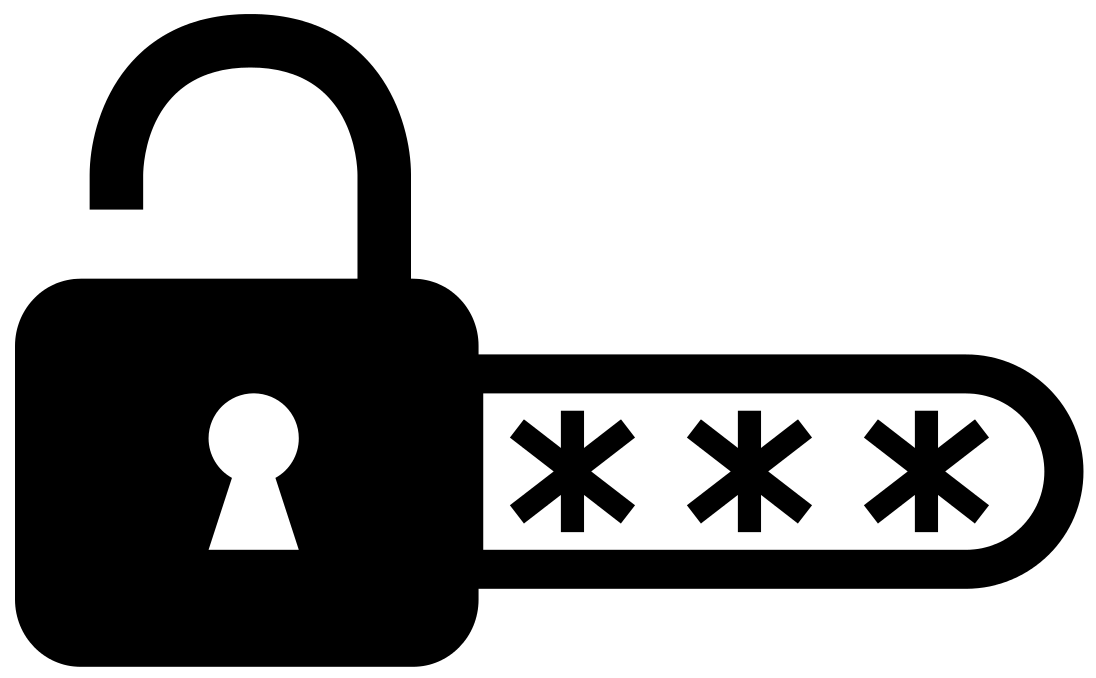
\includegraphics[width=0.2\textwidth]{password}};
          \node[circle,draw,fill=gray,minimum width=4cm,anchor=215]
          (have) at (0,1) {
            
\includegraphics[height=0.2\textwidth]{phone}};
          \node[circle,draw,fill=gray,minimum width=4cm,anchor=90]
          (are) at (0,1) {
            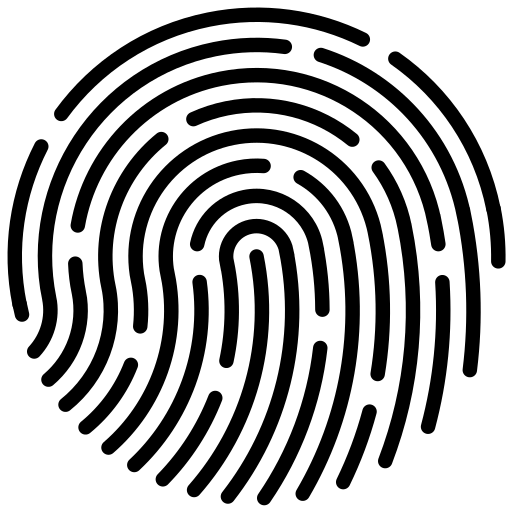
\includegraphics[height=0.2\textwidth]{touch-id}};
        \end{scope}
      \end{tikzpicture}
      \caption{Different possibilities for 2FA Methods
        \endnote{\url{https://www.pngegg.com/en/png-eyxan}}
        \endnote{\url{https://images.vexels.com/media/users/3/157570/isolated/lists/4b39b362c76ea5a00de62f8ff839b5ed-einfaches-smartphone-symbol.png}}
        \endnote{\url{https://cdn4.iconfinder.com/data/icons/apple-touch-id/512/Touch_ID-512.png}}
      }
    \end{figure}
  \end{center}

  \note{
    \begin{itemize}
      \item seem to already know what 2 Factor Authentication is\ldots
      \item 2 Factor Authentication, also abreviated with 2FA requires user to present 2 of 3 authentication factors
      \item These are
            \begin{itemize}
              \item something you know \textrightarrow{} most of the times a password
              \item something you have \textrightarrow{} a phone or an additional device
              \item something you are \textrightarrow{} fingerprint or iris scan
            \end{itemize}
      \item Combination of 2 different factors \textrightarrow{}
    \end{itemize}
  }
\end{frame}
